%-----------------------------QUESTÃO------------------------------------
%Cód.: TF3p24q06


\question Determine a intensidade do campo elétrico criado por
uma carga pontual $q$ de \SI{-8,0e-6}{\coulomb}, em um ponto A situado a \SI{6,0e-2}{\centi \meter} (6 centímetros)
dessa carga. \\
Dados:\\
Constante eletrostática do vácuo $k=\SI{9e9}{\newton\meter^2\per\coulomb^2}$\\
Força Elétrica: $E=k\times\frac{ q }{d^{2}} 
				$

%------------------------------ALTERNATIVAS-----------------------------

		\begin{EnvUplevel}
			\begin{choices}
			
			\choice \SI[per-mode = symbol]{6,0e5}{\newton\per\coulomb}  
			\choice \SI[per-mode = symbol]{2,0e4}{\newton\per\coulomb}
			\choice \SI[per-mode = symbol]{4,0e7}{\newton\per\coulomb}
			\correctchoice \SI[per-mode = symbol]{2,0e7}{\newton\per\coulomb}
			\choice \SI[per-mode = symbol]{7,0e7}{\newton\per\coulomb}
				
			\end{choices}
		\end{EnvUplevel}

%--------------------------SOLUÇÃO---------------------------------------
		
		\begin{EnvUplevel}
		\begin{solution}
		{\footnotesize
		Como as cargas têm sinais opostos, a interação entre elas é atrativa.
		
		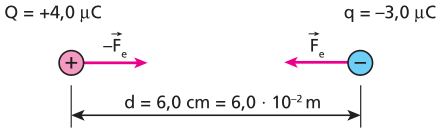
\includegraphics[width=0.4\linewidth]{questoes/imagens/TF3p05q24_1}
	
		Aplicando a Lei de Coulomb a essa interação, temos:
				$$
				F_e=k\times\frac{\left| Q \times q \right|}{\left( d \right)^{2}} \\
				$$
		Substituindo os valores conhecidos, vem:
				$$
				F_e=\num{9e9}\times\frac{\left| \num{4,0e-6} \times \num{3,0e-6} \right|}{\left( \num{6,0e-2} \right)^{2}}
				$$
				$$
				F_e=\SI{30}{\newton}
				$$
		}
		
		\end{solution}
		\end{EnvUplevel}
